\documentclass[aspectratio=169]{beamer}
\usetheme{Madrid}
\usecolortheme{beaver}
\usepackage{tikz}
\usetikzlibrary{positioning, arrows.meta}
\usepackage{booktabs}

\definecolor{amdred}{HTML}{ED1C24}
\definecolor{okgreen}{HTML}{1A7F37}
\setbeamercolor{structure}{fg=amdred}
\setbeamercolor{title}{fg=white,bg=amdred}
\setbeamercolor{frametitle}{fg=white,bg=amdred}

\title{Smart Router}
\subtitle{Track 1 --- General-Purpose AI Agent}
\author{Wilfred Dor\'e}
\institute{AMD Developer Hackathon --- ACT II}
\date{July 2026}

\begin{document}

\begin{frame}
  \titlepage
  \begin{center}
    \texttt{ghcr.io/wilfred-dore/track1-smart-router:latest}
  \end{center}
\end{frame}

\begin{frame}{The problem: accuracy is a gate, tokens are the score}
  \begin{columns}[T]
    \column{0.55\textwidth}
      \textbf{Enterprise reality}
      \begin{itemize}
        \item Not every task deserves a premium model
        \item Host cheap local models in-house, call the paid API only when it matters
        \item Track 1 scores exactly that: pass the 80\% accuracy gate, then rank by \textbf{fewest Fireworks tokens}
      \end{itemize}
    \column{0.4\textwidth}
      \textbf{Consequences for design}
      \begin{itemize}
        \item Local inference = 0 tokens $\Rightarrow$ use it aggressively
        \item Every escalation must be \emph{deliberate}
        \item Extra accuracy above the gate is wasted tokens
      \end{itemize}
  \end{columns}
  \vspace{0.4cm}
  \centering
  \small 8 task categories: factual QA $\cdot$ math $\cdot$ sentiment $\cdot$ summarization $\cdot$ NER $\cdot$ code debugging $\cdot$ logic $\cdot$ code generation
\end{frame}

\begin{frame}{Architecture: a single-pass cascade, never a loop}
  \centering
  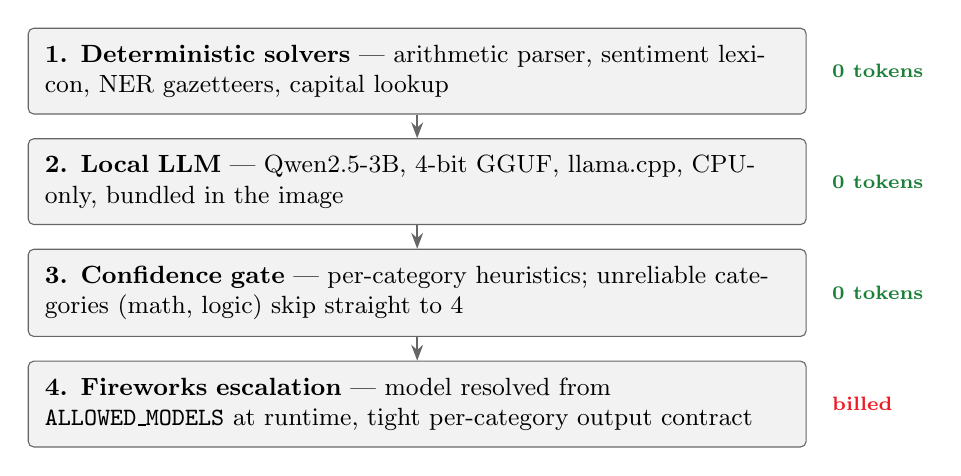
\begin{tikzpicture}[
    node distance=3mm,
    stage/.style={rectangle, rounded corners=2pt, draw=black!60, fill=black!5,
                  text width=0.78\textwidth, align=left, inner sep=6pt, font=\small},
    cost/.style={font=\scriptsize\bfseries},
    arrow/.style={-{Stealth[length=2mm]}, thick, black!60}
  ]
    \node[stage] (s1) {\textbf{1. Deterministic solvers} --- arithmetic parser, sentiment lexicon, NER gazetteers, capital lookup};
    \node[stage, below=of s1] (s2) {\textbf{2. Local LLM} --- Qwen2.5-3B, 4-bit GGUF, llama.cpp, CPU-only, bundled in the image};
    \node[stage, below=of s2] (s3) {\textbf{3. Confidence gate} --- per-category heuristics; unreliable categories (math, logic) skip straight to 4};
    \node[stage, below=of s3] (s4) {\textbf{4. Fireworks escalation} --- model resolved from \texttt{ALLOWED\_MODELS} at runtime, tight per-category output contract};
    \node[cost, right=2mm of s1, okgreen] {0 tokens};
    \node[cost, right=2mm of s2, okgreen] {0 tokens};
    \node[cost, right=2mm of s3, okgreen] {0 tokens};
    \node[cost, right=2mm of s4, amdred] {billed};
    \draw[arrow] (s1) -- (s2);
    \draw[arrow] (s2) -- (s3);
    \draw[arrow] (s3) -- (s4);
  \end{tikzpicture}
\end{frame}

\begin{frame}{Engineering for the grading environment}
  \begin{itemize}
    \item \textbf{Everything config-driven} --- gate thresholds, category$\to$model mapping, token budgets, escalation policy. No hardcoded answers, no caching across runs.
    \item \textbf{Reasoning-model safety} --- inline \texttt{<think>} blocks stripped; if thinking consumes the whole token budget, the answer is recovered from the reasoning field instead of returning empty.
    \item \textbf{Graceful degradation} --- a broken local runtime falls back to full escalation; the container never crashes, every \texttt{task\_id} always gets an answer.
    \item \textbf{Mock mode} --- the full pipeline runs and counts tokens without any API key; \texttt{auto} mode switches to live when the harness injects credentials.
    \item \textbf{Calibrated by sweep, not by hand} --- routing policies compared on a 19-task local eval (8 official practice tasks + 11 self-authored variants).
  \end{itemize}
\end{frame}

\begin{frame}{Results --- measured in CI under the exact grading limits}
  \centering
  \begin{tabular}{lll}
    \toprule
    \textbf{Metric} & \textbf{Measured} & \textbf{Constraint} \\
    \midrule
    Runtime, 19 tasks (4 GB RAM, 2 vCPU, amd64) & 90 s & 600 s \\
    Compressed image size & 1.97 GB & 10 GB \\
    Estimated Fireworks tokens / full run & $\sim$900 & leader: 4{,}268 \\
    Local eval accuracy (escalations assumed) & 19/19 & gate: 16/19 \\
    Output schema \& exit code & valid & required \\
    \bottomrule
  \end{tabular}
  \vspace{0.5cm}
  \begin{itemize}
    \item CI pipeline: native amd64 build $\to$ smoke test at grading limits $\to$ size check $\to$ publish
    \item The smoke test already caught one real bug (musl-linked wheel) before any submission slot was spent
  \end{itemize}
\end{frame}

\begin{frame}{Takeaways}
  \begin{itemize}
    \item \textbf{Zero-cost first}: solvers + a bundled 3B handle most of the load; the paid API sees only the hard residue
    \item \textbf{Route by reliability, not by difficulty}: categories where a small model fails \emph{silently} (math, logic, multi-part factual) escalate outright
    \item \textbf{Plumbing wins hackathons}: most failed submissions break on infrastructure --- CI reproduces the grading environment exactly
  \end{itemize}
  \vspace{0.6cm}
  \centering
  \structure{\textbf{Submission}}\\[2mm]
  \texttt{ghcr.io/wilfred-dore/track1-smart-router:latest}\\[1mm]
  \small public $\cdot$ linux/amd64 $\cdot$ weights bundled $\cdot$ no secrets inside
\end{frame}

\end{document}
